\chapter{Logarithmic Functions}
%%%%%%%%%%%%%%% SECTION HEADER %%%%%%%%%%%%%%%%
\rhead{2}
\lhead{Logarithmic Functions}
%%%%%%%%%%%%%%%%%%% START %%%$%%%%%%%%%%%%%%%%%
\section{What is logarithm?}
Logarithm are-at the most basic level-invented to avoid very large numbers. It was first
introduced by\textit{John Napier} in 1614. As a matter of fact, a logarithm is an
operation that can be applied on a number and return its exponent; In other words,
logarithm is always equal to an exponent. \[
								Logarithm = Exponent
											\]  
Logarithm is denoted as log. If I asked you what is the $2^4$, I am actually asking you 
to use the exponential function to calculate that statement. We all know that 
$2^4=2\cdot2\cdot2\cdot2\cdot=16$. Nonetheless, in Logarithm realm, we asked inversely. 
"What power should I raised base 2 to get 16"? In other words,\[
								2^? = 16
											\]
We know the answer to this question is 4. Using Logarithm, we can rewrite this question 
into			\[
						\log_{2}16 =?				
				\]
Notice the base 2 is written as a subscript. You can read it as “log base 2 of 16”. 
	\begin{tcolorbox}[title=Logarithmic function, 
	                fonttitle=\bfseries,
	                colframe=blue!70!black,
	                colback=white]
		For $x>0$ and $b>0$, $b\neq1$,
		\begin{equation}
			\log_{b}x=y\quad \text{is equivalent to}\quad  b^y=x
			\label{log}
		\end{equation}
		The function $f(x)= log_{b}x$ is the logarithmic function with base b.
	\end{tcolorbox}
Figure \ref{fig:log} is showing each component of logarithms:
		\begin{figure}[H]
		 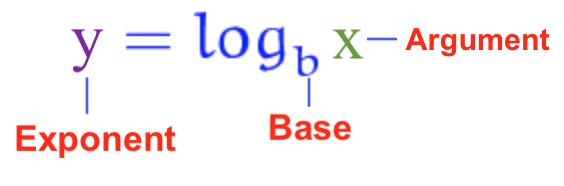
\includegraphics[width=5cm]{pics/Log.png}
		 \centering
		 \caption{Components of a log}
		 \label{fig:log}
		\end{figure}
A good way to remember how log works, draw an arrow as shown in Figure \ref{fig:log_arrows}. Raise $b$ to the power of $y$ to obtain $x$.
		\begin{figure}[H]
		 \centering
		 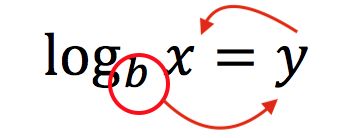
\includegraphics[width=0.25\textwidth]{pics/log_arrow.png}
		 \caption{Arrows help us to convert logarithmic form to exponential form}
		 \label{fig:log_arrows}
		\end{figure}
% ========== FACT
\begin{fact}
Logarithm gives us an exponent whereas exponential function will raise the base to 
that exponent; In other words, logarithm and exponential functions are undoing each 
other. Consequently, they are inverse of each other.
\end{fact}
% ============== EXMP 1
\begin{exa}
	Write each equation in its equivalent exponential form.
	\begin{multicols}{3}
	\begin{enumerate}[\bfseries a.]
		\centering
		\item $3= \log_{7}x$	
		\item $2= \log_{b}25$
		\item $\log_{4}26=y$
	\end{enumerate}
	\end{multicols}
\end{exa}
Using the definition of log, equation \eqref{log}, we can rewrite them in their 
exponential form.\\[1cm]
a.
\begin{align*}
	  3 =\log_{7}x&  &&\text{Use the definition of log}\\
	7^3 =x&	&&\text{Our solution}
\end{align*}
b.
\begin{align*}
	  2 =\log_{b}25&  &&\text{Use the definition of log}\\
	b^2 =25&	&&\text{Our solution}
\end{align*}
c.
\begin{align*}
	\log_{4}26 =y&  &&\text{Use the definition of log}\\
	26 =4^y&	&&\text{Our solution}
\end{align*}
% ============== EXMP 2
\begin{exa}
	Write each equation in its equivalent logarithmic form.
	\begin{multicols}{3}
	\begin{enumerate}[a.]
		\centering
		\item $2^5=x$	
		\item $b^3=27$
		\item $e^y=33$
	\end{enumerate}
	\end{multicols}
\end{exa}
a.
\begin{align*}
	  2^5 &=x  &&\text{Recall $log=exponent$, We know base is 2}\\
	\log_{2}x &=5	&&\text{Our solution}
\end{align*}
b.
\begin{align*}
	  b^3 &=27  &&\text{Using $log=exponent$, We know base is b}\\
	\log_{b}27 &=3	&&\text{Our solution}
\end{align*}
c.
\begin{align*}
	e^y &=33  &&\text{Using $log=exponent$, We know base is $e$}\\
	\log_{e}\,33 &=y	&&\text{Our solution}
\end{align*}
% =========== SECTION
\section{Evaluating logarithm without using calculator}
By using the definition of logarithm, we can find the value of some logarithms. For 
example, to find $log_{3}81$, we should ask ourselves, “3 to what power gives 81?” In 
other words, \[
				3^?=81
				\]
It is obvious that the answer is 4 because $3^4=81$. Therefore $\log_{3}81=4$. In next 
section, you will see that product rule makes it much easier to evaluate such logarithms.
% ============== EXAMPLE 3
\begin{exa}
    Without using the calculator evaluate each logarithm:
    \begin{multicols}{2}
	\begin{enumerate}[a.]
		\centering
		\item $\log_{10}100$	
		\item $\log_{5}\frac{1}{125}$
		\item $\log_{36}6$
		\item $\log_{3}\sqrt[7]{3} $
	\end{enumerate}
	\end{multicols}
\end{exa}
%
a. \begin{align*}
	  \log_{10}100 =?&  &   &\text{10 to what power gives 100?}\\
	  2&	&   &\text{Our Solution}
\end{align*}
%
b. \begin{align*}
	  \log_{5}\frac{1}{125}=?&  &       &\text{$\frac{1}{125}$ is equal to $5^{-3}$}\\
	  &&							    &\text{5 to what power gives $5^{-3}$?}\\
	  -3& 	&   &\text{Our Solution}
\end{align*}
%
c. \begin{align*}
	  \log_{36}6 =?&            &       &\text{36 to what power gives 6?}\\
	  \frac{1}{2}&          	&       &\text{Our solution}
\end{align*}
%
d. \begin{align*}
	  \log_{3}\sqrt[7]{3}=?&       &   &\text{$\sqrt[7]{3}$ is equal to $3^{1/7}$}\\
	  &&						       &\text{3 to what power gives $3^{1/7}$?}\\
	  \frac{1}{7}&	&                  &\text{Our Solution}
\end{align*}
% ======== NOTE
\begin{nt}
    In next section, you will see that power rule property will help us find this type of logarithms easily.  
\end{nt}
% ============ SECTION
\section{Common and natural logarithm}
In mathematics, we love number 10 (why?). Euler number also appears in a lot of problems.
That's why most of the time, our bases are either 10 or $e$. 
	\begin{tcolorbox}[title=log and ln, fonttitle=\bfseries,
	                  colframe=blue!75!black,
	                  colback=white]
		\begin{itemize}
			\item $\log_{10}x$ is written as "$\log_{}x$" and is called common logarithm.
			\item $\log_{e}x$ is written as "$\ln{x}$" and is called natural logarithm.
		\end{itemize}
	\end{tcolorbox}
\section{Identity and inverse properties}
We know that $a^1=a$. We can rewrite this expression in logarithmic form, using
\eqref{log}, and we will get \begin{equation}
								\log_{a}a=1 \label{ID_1}					
							\end{equation}
Likewise, we must know that $a^0=1$, and by using \eqref{log}, we have 
							\begin{equation}
								\log_{a}1=0 \label{ID_2}
							\end{equation}
These two properties are called \textit{identity properties}-because we are having number 
1.\\
As we discussed earlier, we realized that exponential and logarithmic functions are
inverse of each other. Here we can prove it easily. First we know that exponential 
function is a one-to-one function, so it must have an inverse. Let's consider $f(x)=a^x$,
		\begin{align*}
		y &= a^x	&	&\text{Switch $x$ and $y$}\\
		x &= a^y	&	&\text{We need to solve for $x$, $x$ is an exponent}\\
		&&&\text{Use definition of log, equation \eqref{log}}\\
		\log_{a}x&=y	&	&\text{replace $y$ with $f^{-1}(x)$}\\
		\log_{a}x&=f^{-1}(x)	& &\text{}
		\end{align*}
Thus, inverse of exponential function is logarithmic function and because they both undo 
each other, we have
		\begin{align}
		f\left(f^{-1}\left(x\right)\right) &= x \label{INV_1} \\
		f^{-1}\left(f\left(x\right)\right) &= x \label{INV_2}	
		\end{align}
Considering $f(x)=a^x$ and $f^{-1}(x)=log_{a}x$, we will get
		\begin{align}
		a^{\log_{a}x} &= x \label{alogax} & &\text{Using property \eqref{INV_1}}\\
		\log_{a}(a^{x}) &= x \label{logaa} & &\text{Using property \eqref{INV_2}}
		\end{align}
%
    These simple properties make us to find some logarithm without using calculator. Table \ref{tab:identity_inverse_table} summarize identity and inverse properties for any positive base, $a>0$:
	\begin{table}[H]
	\centering
	\caption{Identity and inverse properties}
	\begin{tabular}{c c c}
	    \toprule
		Identity properties        & & Inverse properties \\
		\hline \hline\\
		$\log_{a}a=1$	& &	$\displaystyle a^{\log_{a}x} = x$	\\ [.5cm]
		$\log_{a}1=0$	& &	$\displaystyle \log_{a}(a^{x}) = x$ \\[.2cm]
		\bottomrule
	\end{tabular}
	\label{tab:identity_inverse_table}
	\end{table}
%
We can also use identity and inverse properties for common and natural logarithm by changing the base to 10 and $e$, respectively. Table \ref{tab:intro_log_ln} shows these properties using log and ln.
	\begin{table}[H]
	\centering
	\caption{Identity and inverse properties using common and natural log}
	\begin{tabular}{c c c}
	    \toprule
		Common logarithm & & Natural logarithm\\
		\hline \hline \\
		$\log_{}10=1$	&	& $\ln{}e=1$	\\[.4cm]
		$\log_{}1=0$	&	& $\ln{1}=0$ \\[.4cm]	
		$\displaystyle 10^{\log_{}x} = x$ & & $\displaystyle e^{\ln{x}} = x$ \\[.4cm]
		$\displaystyle \log_{}10^{x} = x$ & & $\displaystyle \ln{e^x} = x$ \\[.4cm]
		\bottomrule
	\end{tabular}
	\label{tab:intro_log_ln}
	\end{table}
% ============== EXAMPLE 4
\begin{exa}
    Evaluate each logarithm:
    \begin{multicols}{2}
    \begin{enumerate}[\bfseries a.]
        \item $\log_{9}9$
        \item $\log_{8}1$
    \end{enumerate}
    \end{multicols}
\end{exa}
Using identity properties, we will get
	\begin{align*}
		\log_{9}9=1 & &\text{Identity property \eqref{ID_1}}\\
		\log_{8}1=0 & &\text{Identity property \eqref{ID_2}}
	\end{align*}

%=============
\section{Graph of Logarithmic Functions}
To sketch the graph of $y=\log_{a}x$, you can use the fact that the graphs of inverse
functions are reflections of each other in the line $y=x$. As you can observe, the $x=0$ 
is a vertical asymptote.
		\begin{figure}[H]
		 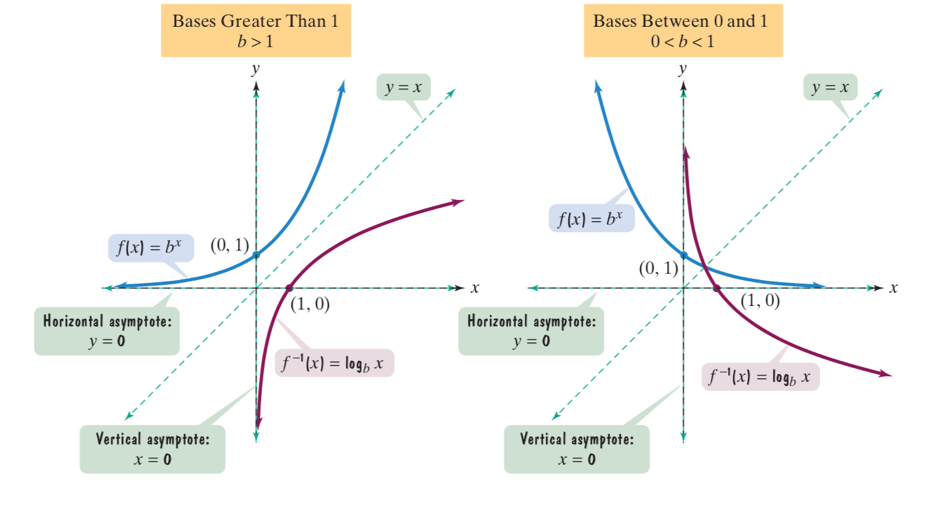
\includegraphics[width=12cm]{pics/log_vs_exp.png}
		 \centering
		 \caption{The Graph of exponential and logarithmic functions}
		 \label{fig:log_vs_exp}
		\end{figure}

You can also plot each logarithmic graph by constructing a table of values and 
connecting points. 
\begin{tcolorbox}[title=Characteristics of $\displaystyle \bm{y=log_{a}x}$,         
                    fonttitle=\bfseries,
                    colframe=red!70!black,
                    colback=white]
	\begin{itemize}
		\item The domain is $(0,+\infty)$	
		\item The range is $(-\infty,+\infty)$
		\item The $x$-intercept is $(1,0)$
		\item $x=0$ is a vertical asymptote
	\end{itemize}
\end{tcolorbox}
\subsection{Domain of logarithmic function}
When determining domain, it is important to determine where the function would not exist.
Regarding logarithmic function, we can only take the logarithm of values greater than 0.
In other words, if we have $f(x)=log_{a}(g)$, therefore the domain of this
function consists of all $x$ for which $g>0$.
% ===== EXAMPLE
\begin{exa}
Find the domain of each function.
 \begin{multicols}{2}
 \begin{enumerate}[\bfseries a.]
    \item $f(x) = \log_{4}(x-5)$
    \item $g(x) = \ln{(4-x)}$
    \item $h(x) = \ln{x^2}$
 \end{enumerate}
 \end{multicols}
\end{exa}
% 
a.\begin{align*}
		f(x) = \log_{4}(x-5)&    &	&\text{$(x-5)$ should be positive} \\
		x-5 > 0&	    & &\text{Solve for $x$}\\
		x>5&    	& &\text{Our domain }\\
		(5,+\infty)&    &   &\text{In interval notation}
\end{align*}
b.\begin{align*}
		g(x) = \ln{(4-x)}& &	&\text{$(4-x)$ should be positive} \\
		4-x > 0&	& &\text{Solve for $x$}\\
		4>x&	& &\text{Our domain} \\
		(-\infty,4)&    &   &\text{In interval notation}
\end{align*}
c.\begin{align*}
		h(x) = \ln{x^2}&     &	    &\text{$x^2$ should be positive} \\
		x^2 > 0&    	&           &\text{Solve for $x$}\\
		x>0\quad or x<0&        &   &\text{Our domain} \\
		(-\infty,0) \cup (0,+\infty)&   &   &\text{In interval notation}
\end{align*}
% ===== EXAMPLE 
\begin{exa}
The percentage of adult height attained by a boy who is $x$ years old can be modeled by 
							\[
							f(x) = 29 + 48.8\log_{}(x + 1)
							\]
where $x$ represents the boy’s age (from 5 to 15) and $f(x)$ represents the percentage of 
his adult height. Approximately what percentage of his adult height has a boy attained at 
age ten? 
\end{exa}
Substitute the boy’s age, 10, for $x$ and evaluate the function.
\begin{align*}
	f(10) &= 29 + 48.8\log_{}(10 + 1) \\
	f(10) &= 29 + 48.8\log_{}(11) \\
	f(10) &= 29 + 48.8(1.04139) \\
	f(10) &= 79.819832 \approx 80 \\
\end{align*}
A 10-year-old boy has attained approximately 80\% of his adult height.